\section{Body of the report}

\subsection{Structure and sections}

The structure of the report and the titles of sections depend on the nature of the project. Here are suggestions for two extreme types, which can be adjusted to suit your report.

\subsubsection{Research projects}

Here you are given a starting point and a general direction: your aim is to discover something new. The report would probably be divided into sections with familiar titles.
\begin{itemize}
\item
\textbf{Theory} -- 
Explain essential background theory that is vital to understand your report. Select and present the material to show its relevance to the project and demonstrate your understanding. Do not repeat standard material from textbooks, which is a waste of space; give a reference instead. 
%Detailed mathematical derivations should be left to an appendix.

\item
\textbf{Experimental Techniques} --
Give an account of your experimental (or numerical) techniques. Emphasise details that would be necessary to continue the work or to compare your results with those of other experimenters. Aim to include what you would have liked to know at the start of your project.

\item
\textbf{Results} --
Describe these at an appropriate level of detail to support your conclusions. Lengthy tables should be left to an appendix or supplied on a CD. Avoid unnecessary detail: describe preliminary experiments briefly if at all, unless they illustrate some important point.
\end{itemize}


\subsubsection{Design, build and test projects}

Here the goal is specified, more or less precisely: your job is to work out how to get there. The titles of the sections are less standardised but here is a possible approach.
\begin{itemize}
\item
\textbf{Specification} --
Typically you are given only a vague description of the functions required and must first develop this into a firm specification against which your final product will be judged.
\item
\textbf{Possible strategies} --
Evaluate \emph{briefly} the possible approaches that you considered 
%for the overall design 
and explain why you selected one of these. 
Avoid excessive detail of discarded possibilities.
\item
\textbf{Implementation} --
Describe the final product. Concentrate on key features that required advanced design and skim over well-known aspects. Mention useful points that might help future students, such as tricky sections of data sheets.

\textbf{Software} is tricky. Often the best approach is to describe the high-level structure in the main text (a diagram of a state machine for example) and pick out any special features of the program. A complete listing should be included as an appendix or on a CD.
\item
\textbf{Testing} --
This is equivalent to the `Results' section of a research project. 
%and the same comments apply.
\end{itemize}


\subsection{Style of writing}

One of the most difficult aspects of writing is to judge the level and background of your readers. Typically the report will be assessed by your first supervisor, who is an expert on the topic, and your second supervisor, who is not. You should therefore assume that the reader is a \emph{well-educated, graduate engineer} but not an expert on the subject of the project. Assume that he or she is familiar with the general concepts taught in courses up to level 3 but not with the details of specialised courses at higher levels.

It is also difficult to appreciate that most readers are not interested in the nitty-gritty detail. They want to know \emph{what} you did and \emph{why} you did it that way but they don't want a step-by-step account of \emph{how} you did it. Your watchword should therefore be:
\begin{center}
\textbf{SUMMARISE!}
\end{center}
Of course some people need the details -- a person continuing work on the project requires precise experimental methods, for instance. Such material may be better in an appendix. The same is true for computer programs and schematics of complicated circuits. Design-and-build projects may need a User's Manual, which should be included as an appendix. 

A report is a formal document and should be written in appropriate language. Numerous books offer advice on writing reports and a selection \cite{jve05,mkm06,dfb09,tmy05} is listed in the references at the end. Here are a few tips.
\begin{itemize}
\item
Reports should be written in correct English. Break text into paragraphs, keep sentences to a reasonable length and insert appropriate punctuation. Use a spell-checker and a grammar-checker if desired but neither is a substitute for careful reading. 
\item
A report is not a story. 
%Write `The transistor exploded', not `I blew up the transistor'. Similarly, 
Write `The voltage was measured' rather than `I measured the voltage'. This document contains instructions and therefore uses a different style.
\item
Define all abbreviations when they are first used: `The accelerometer uses a serial peripheral interface (SPI)'. Provide a list of abbreviations if you use a large number of them.
\item
Don't write material that you don't understand. It will be obvious to the reader.
\end{itemize}
The quality of English is assessed as part of the report. Foreign students may feel this to be a burden but part of their education in this country is to learn to work effectively in an English-speaking environment. 

\subsection{Precision}

An engineering report must be precise. This applies both to the language and to numerical values. For example, the words \emph{precision} and \emph{accuracy} are often used interchangably in non-technical discussion but the distinction between them is vital in engineering.

Quote numerical results to an appropriate number of significant figures. For example, it is pointless to claim that a length was 12.345\,mm if it was measured with a pocket ruler. Don't simply write down all the digits displayed on your calculator. 

Analyse the uncertainties in your results to increase the impact of your results. Please avoid horrors like this:
\begin{quote}
The gain was quite accurate.
\end{quote}
The sentence is meaningless and the reader will doubt whether you have any idea of the accuracy. Contrast this sentence:
\begin{quote}
The accuracy of the gain was estimated to be $\pm 2\%$, limited by the tolerance of the resistors. A detailed analysis is given in Appendix C.
\end{quote}
This is informative and convinces the reader that you have a full understanding.

\subsection{Figures and tables}

\begin{figure}
\centering
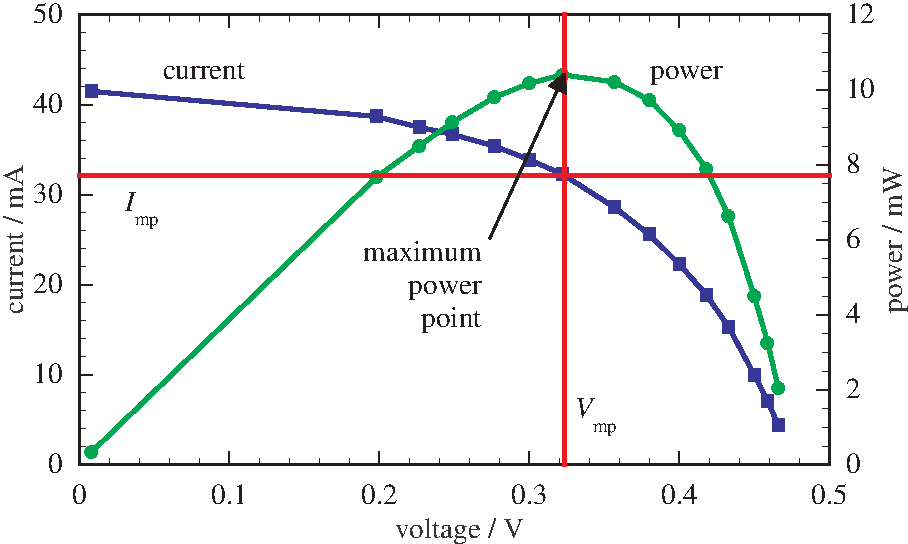
\includegraphics[scale=0.72]{solarcell}
\caption{Current and power as a function of voltage delivered by a single photovoltaic cell under illumination from a 150\,W metal halide floodlamp, showing the maximum power point.}
\label{solar cell fig}
\end{figure}

Figures and tables must have informative captions and be numbered as in Figure~\ref{solar cell fig}. Axes of graphs should have scales, titles and units, otherwise the plot is meaningless. All text must be legible, roughly the same size as the main text. Be warned that plots from Excel need extensive editing to bring them up to an acceptable standard. Oscilloscope screenshots can make good illustrations and are simple to capture on modern equipment.

Tables must have appropriate headings with units. Avoid lengthy tables: consider whether a graph would be clearer or the data would be better on a CD.

\subsection{References}

No project is done in isolation. A research project builds on the results of previous workers; a design-and-build project depends on the properties of the components available. You therefore draw on published documents during your project and must provide \emph{references} to these sources in your report. References are cited (a)~to give due credit to the originator and (b)~to guide a reader who wants more detailed information. You should give a reference wherever it is required for either of these purposes. Properly referenced material from many sources is a sign of a good project report. 
%This section explains how to present such references and how you will be penalised if you fail to do this. The mark for the report include an element for references to reflect their importance.

References must be cited with sequential numbers in square brackets where they are used in the text, not just listed at the end of the report. Typical usage is `Fitzmaurice and Hand \cite{gmf87} showed that\dots' or `The median is an appropriate estimator for this signal \cite{gmf87}'.

Avoid direct quotations from references in general; make it absolutely clear that the text is a quotation if this is unavoidable. An illustration, such as a diagram from a data sheet, is another type of quotation and must be referenced, typically in the figure caption. This is perfectly acceptable: do not waste time redrawing diagrams.

\subsubsection{Plagiarism}

If you copy from another person's work (project report, book, journal, web page or any other document) without acknowledging the source, you are guilty of \emph{plagiarism}. This is a disciplinary offence and the University has procedures for handling it. The failure to acknowledge a source is considered as plagiarism even if there was no deliberate intention to cheat. 

Avoid any risk of plagiarism by providing a reference for all sources that you use. Read the advice offered by the University Library and consult your supervisor if you are in any doubt. The University's \emph{Plagiarism Statement} is reproduced in Appendix \ref{plagiarism sect}.

\subsubsection{List of references}

All reports must have a section entitled `References' after the main text but before any appendices. This comprises a list of references, numbered to match the citations in the text. Each reference requires the following information and the cited references provide examples.
\begin{itemize}
\item
\textbf{Journal paper}: 
author(s), title of paper, name of journal, volume number, first page, last page and year \cite{gmf87}. 
Many journals now use article numbers instead of page numbers.
\item
\textbf{Book}: 
author(s), title, edition, publisher and year of publication \cite{jve05}.
Include the number of the chapter or page(s) if you refer to only a small part of the book.
\item
\textbf{Data sheet}: 
company, title, edition and date \cite{s08qg}. 
Application notes, technical reports and similar documents should be cited in the same way.
\item
\textbf{Web page}: 
author(s) or organisation, title, full URL and date of viewing \cite{mac09}. See below.
\end{itemize}
%The general rule is that 
The reader must be able to find the document without searching for further information.

\subsubsection{References from the Web}

The World Wide Web is a wonderful resource because it is so easy to search. It is therefore tempting to use web pages as references. \emph{Proceed with caution} because the accuracy of many web sites cannot be verified. This is particularly true for anonymous sites such as Wikipedia. Use them only as a starting point: good pages provide references to more authoritative sources.

Reports whose references are all or mainly from the web, especially from anonymous sites, will be penalised.
